\documentclass[12pt]{article}
\usepackage{fullpage} 
\usepackage{microtype}      % microtypography
\usepackage{array}
\usepackage{amsmath,amssymb,amsfonts}
\usepackage{amsthm}
\usepackage{graphicx}
\usepackage{caption}

%% Header
\usepackage{fancyhdr}
\fancyhf{}
\fancyhead[C]{CS 136 - 2022s - Checkpoint 2}
\fancyfoot[C]{\thepage} % page number
\renewcommand\headrulewidth{0pt}
\pagestyle{fancy}

\usepackage[headsep=0.5cm,headheight=2cm]{geometry}

%% Hyperlinks always blue, no weird boxes
\usepackage[hyphens]{url}
\usepackage[colorlinks=true,allcolors=black,pdfborder={0 0 0}]{hyperref}

%%% Doc layout
\usepackage{parskip}
\usepackage{times}

%%% Write out problem statements in blue, solutions in black
\usepackage{color}
\newcommand{\officialdirections}[1]{{\color{blue} #1}}

%%% Avoid automatic section numbers (we'll provide our own)
\setcounter{secnumdepth}{0}

%%% Figure settings
\captionsetup[figure]{labelfont=bf,textfont=it}

\begin{document}
~~\\ %% add vert space

\begin{center}
{\Large{\bf Student Names: Nate Davis and Alexander Lobo}}
\end{center}

~~\\ %% add vert space

{\Large{\bf Collaboration Statement:}}

Turning in this assignment indicates you have abided by the course Collaboration Policy:

\url{www.cs.tufts.edu/comp/136/2022s/index.html#collaboration-policy}

Total hours spent: 10-15

We consulted the following resources:
\begin{itemize}
\item Wikipedia
\item Stack Overflow
\item Course Website
\end{itemize}

\tableofcontents

\newpage

\section{Applying Model to Dataset}

For this project, we have decided to implement a Bayesian Logistic regression model to predict the class of conformations of molecules as either "musk" or "non-musk".

We used the \texttt{MAPEstimator.py} class from CP2 as a template to set up our model. In our python file, we have a \texttt{MAPEstimator} class with an initialization (\texttt{\_init\_}). Various methods (\texttt{fit()}, \texttt{predict\_proba()}, and \texttt{score()}) are also implemented to train and test the model. Details of our implementation are below.

\subsection{Initialization}

The \texttt{MAPEstimator} class has the following attributes that are defined in the initialization:

\begin{itemize}
\item \texttt{w\_D} : defines the first instance of the weight vector

	\begin{itemize}
	\item is a vector of all zeros since our prior (both trivial and SAS) assumes a zero mean
	\end{itemize}
	
\item \texttt{prior} : determines which prior to use (\texttt{'trivial'} or \texttt{'sas'}) [Refer to "Upgrades" section for more details]

	\begin{itemize}
	\item \texttt{'trivial'} prior :
\begin{equation}
p(\textbf{w}|\alpha) = \mathcal{N}(\vec{0}, 	\alpha^{-1}I_{166})
\end{equation}
	\item \texttt{'sas'} prior (sas stands for "spike-and-slab"):
\begin{equation}
p(\textbf{w}|\alpha,\beta) = 0.8\mathcal{N}(\vec{0}, 	\alpha^{-1}I_{166}) + 0.2\mathcal{N}(\vec{0}, 	\beta^{-1}I_{166})
\end{equation}
	\end{itemize}

\item \texttt{alpha} : A real value that determines the precision of either the trivial prior or first MVN in the SAS prior

\item \texttt{beta} : A real value that determines the precision of the second MV in the SAS prior (should only be specified if \texttt{prior='sas'}

\item \texttt{max\_iter} : A positive integer that determines the maximum number of iterations allowed for the stochastic gradient descent

\item \texttt{tol} : A real positive value that determines the tolerance for convergence for the stochastic gradient descent

\item \texttt{step\_size} : A positive real value that determine how large the weight update is per iteration

\end{itemize}

\subsection{Training}

The \texttt{fit()} method is used to train the Bayesian logistic regression model with the provided training data. Since stochastic gradient descent is being used, a while loop iterates over each training example to compute the gradient of the posterior distribution. This gradient is then used to update to update the weight vector and bias term according to the following equations, where $c$ is the bias term:

\begin{equation}
\mathbf{w}^{t+1} \leftarrow \mathbf{w}^{t} - \eta \left[ \left(\sigma(\mathbf{w}^t \cdot x^{(i)}) - y^{(i)}\right) x^{(i)} + \alpha \mathbf{w}^{t} \right]
\end{equation}

\begin{equation}
c^{t+1} \leftarrow c^{t} - \eta (\sigma(\mathbf{w}^t \cdot x^{(i)}) - y^{(i)})
\end{equation}

After each update, the log loss for that example is computed using the following equation:

\begin{equation}
L = y^{(i)} \log \hat{y}^{(i)}+ (1-y^{(i)})\log(1-\hat{y}^{(i)})
\end{equation}

This loss is then appended to a vector of losses. Since stochastic gradient descent is prone to fluctuations in the loss at each step, after 10 iterations, the previous ten losses are averages and then compared to the 10 before that to see if the average loss change is reducing. If the average loss change becomes less than the tolerance, then it is said to have converged and the loop halts. If the average change in loss does not converge, then the loop halts when the maximum number of iterations are reached.

\subsection{Evaluation}

The \texttt{predict\_proba()} method is used to predict the probability of each example being in the "musk" and "non-musk" class while the \texttt{score()} method uses a threshold of 0.5 to characterize each example and then compute the accuracy of the predictions by comparing to the true class labels. After splitting our data set into a training and testing set and training the model on the training set, we can evaluate the models performance by calculating the prediction score with the testing set. We can also use the \texttt{iter\_count} attribute to evaluate many iterations it took for the training to converge.

\subsection{Bottlenecks}

We decided to first test our model with a learning rate and $\alpha$ value of both 1. However, upon implementation, we noticed that the model would not converge, instead, the loss would shoot up to infinity after a few iterations. We then normalized the data using a standard scaler, assuming that the large feature values were causing large steps in the weight updates. However, this led to the same result. After deliberating, we decided to reduce our step-size to 0.1. After this change, the average loss started decreasing with each iteration started to converge.

As discussed further in our Evaluation section, another bottleneck we have run into is our model's accuracy. After correcting the first issue of convergence, we observed testing accuracies between 50\% and 60\%. Looking at the distribution of the output class imbalance

\begin{figure}[h!]
\begin{center}
  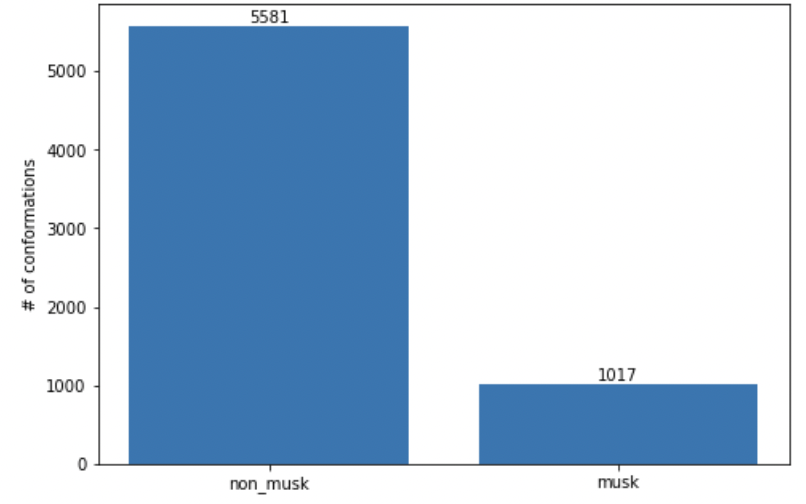
\includegraphics[scale=0.7]{images/outcome_distrib.png}
  \caption{Distribution of examples by output class}
  \label{fig:1}
\end{center}
\end{figure}

we can see that the occurrence of non-musk (\texttt{class=0}) molecules occur about 85\% of the time. This implies that our Bayesian logistic regression model was performing worse than a trivial "always-1" classifier. This trivial model would not implement any machine learning logic and instead would always guess that the output class is a non-musk molecule. Our poor accuracies are indicative of a broader issue with our model that we suspect was due to the class imbalance. How we addressed this issue is elaborated in the next section. Implementing our change improved the accuracy, but not significantly enough to be better than a "always-1" classifier. Unfortunately, we were not able to construct a new solution, although we do suspect that there is either a problem with our weight update formula or that the model is not training well with a stochastic gradient descent algorithm. We might try implementing a batch or mini-batch gradient descent algorithm to see if that improves our accuracy without detriment to our training time and number of iterations. Regardless, we would like to discuss our results and ideas further with Ike to get his opinion.


\section{Evaluating Hypotheses from Checkpoint 1}

We have tweaked our hypotheses from Checkpoint 1. The one that is testable at this stage is now:

\begin{itemize}
    \item We hypothesize that our multivariate logistic regression model with first-order stochastic gradient descent will converge in fewer iterations, but with ultimately similar accuracy, when we use different step sizes for misclassifying the two output classes, as our output classes are highly imbalanced.
\end{itemize}

We evaluated this hypothesis via (shuffled) K-fold cross validation with 10 folds, noting how many iterations it took the model to converge for each fold and the accuracy on the held-out examples. The hyperparameters held fixed across the tests were a prior weight vector of zeros with precision of 0.1, a standard step size of 0.1 and, in the dynamic case, a step size of 0.2 for musks, a convergence tolerance of $10^{-4}$, and a max iteration count of 10,000,000.

The results can be seen below:

\begin{figure}[h!]
\begin{center}
  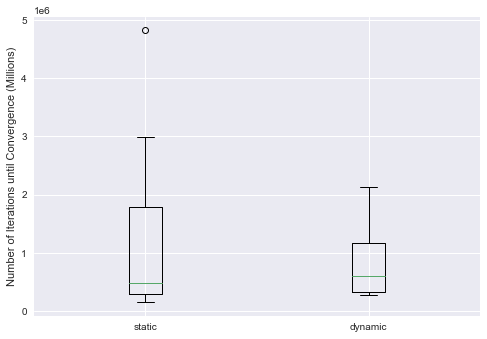
\includegraphics[scale=0.7]{images/iter_counts.png}
  \caption{Training iterations count by weight update scheme}
  \label{fig:2}
\end{center}
\end{figure}

Figure 2 shows the distribution of iteration counts (in millions) for the training of each of the models until convergence. The median of the model trained with dynamic step size is slightly higher than that of the static model, but the variance is much smaller, especially on the high end. The longest the dynamic model took to train was approximately 2 million iterations while the static model has two training runs that took far longer. The interquartile range for the model with dynamic step size is also quite a bit smaller.

\begin{figure}[h!]
\begin{center}
  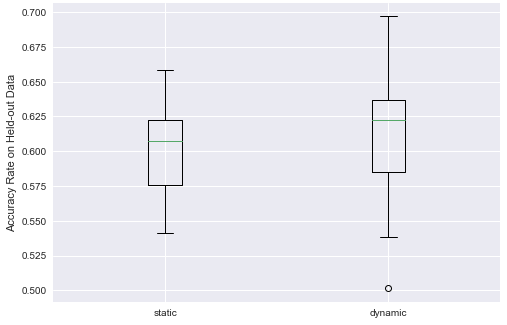
\includegraphics[scale=0.7]{images/accuracy_rates.png}
  \caption{Held-out accuracy rates by weight update scheme}
  \label{fig:3}
\end{center}
\end{figure}

As for accuracy rate, the results are somewhat flipped, with the dynamic step size model having a higher median and interquartile range, but a much larger range of outcomes overall. 

Our hypothesis, which contains two sub-hypotheses, was correct to an extent. The model with dynamic step size certainly seems to have iteration counts that generally cluster around a lower value, but the median value for the static step size is actually smaller. The difference really seems to be more about variance than a representative value.

As for the accuracy rate, we did not foresee the dynamic model performing better than the static, and also said nothing regarding the variance of results. We thought that the models might converge to the same places, but perhaps with the randomness we introduced into the training process, the models reached our (somewhat arbitrary) conversion threshold at different times.


\section{Proposing an Upgrade to your Model or Learning Method}

The purpose of this study is to explore how our model performs when upgrading our
learning method from a first order to a second order gradient descent algorithm to solve the
weight vector MAP estimate for logistic regression. However, considering the issues we had with training convergence and prediction accuracy when testing our model for this checkpoint, we have actually decided to expand our scope to two upgrades.

\textbf{Upgrades:}

\begin{enumerate}
\item Upgrade gradient descent algorithm to obtain the MAP estimate for Bayesian logistic regression from a first-order stochastic gradient descent to a second-second order stochastic gradient descent
\item Upgrade the prior distribution from a "trivial" prior to a "spike-and-slab" prior
\end{enumerate}


Considering both of these upgrades, we propose the following hypotheses
for how we expect our model to perform.

\textbf{Hypotheses:}

\begin{enumerate}
\item We hypothesize that the time and iterations needed to compute the weight vectors will decrease
after upgrading from a first order to second order gradient descent.

\item We hypothesize that our multivariate logistic regression model with both first-order and second-order stochastic gradient descent will converge in fewer iterations when we use a spike-and-slab prior.

\item We hypothesize that our multivariate logistic regression model with second-order stochastic gradient descent will converge in fewer iterations, but with ultimately similar accuracy, when we use different step sizes for misclassifying the two output classes, as our output classes are highly imbalanced.

	\begin{itemize}
	\item Since we were already able to test this hypothesis with first-order gradient descent with positive results, we expect the same to occur with second-order.
	\end{itemize}

\end{enumerate}


\subsection{Upgrade 1: First to Second-Order Gradient Descent}

\subsubsection{Description}
In Bayesian logistic regression, the Posterior distribution is a useful probability distribution to may be used to predict the probability of certain weight vectors given then occurrence of specific data. It is a powerful tool that allows us to utilize information from the Likelihood (probability of data given weight vector), the Prior (a prior knowledge about the weight vector), the Evidence (marginal probability of the data). One goal of Bayesian reasoning for logistic regression is to find the most probable weight vector that maximizes the probability density of the Posterior, which is known as the MAP estimate. However, unlike with linear regression, the MAP estimate of logistic regression is not known to have an analytical solution. Therefore we depend on optimization methods like gradient descent to solve

\begin{equation}
\hat{\textbf{w}}_{\mathrm{MAP}} = \arg\max_{\textbf{w} \in \mathbb{R}^M} \log p(\textbf{w}|\textbf{t}) 
\end{equation} 

We then have two options to choose from: first-order or second-order gradient descent. First order gradient descent uses a first-order derivative of the Posterior to make a step change in the weight vector, while second-order gradient descent uses a second-order derivative.

This upgrade falls under \textbf{Option 3} (Changing the inference method) out those provided.

\subsubsection{Implementation}

To implement this upgrade, we will need to make the following changes to our model:

\begin{itemize}
\item Add an attribute to our initialization to specify the gradient descent method that should be used (e.g. \texttt{solver=\{'fo','so'\}})
\item Create an \texttt{if} statement in the \texttt{fit()} method to update the weights accordingly
\item Write out the math for the second-order gradient descent formula and implement in in the \texttt{fit()} method
\end{itemize}


\subsubsection{Benefit(s)}

It is widely accepted –and stated in the lecture notes– that second-order gradient descent is the "gold standard form MAP estimation". However, unlike linear regression it is not able to converge to the optimal solution in a single step. Regardless, it is expected that that implementing a second order gradient descent for logistic regression MAP estimation greatly reduces the number of iterations needed to converge.

We think that this will not only help reduce the high number of iterations observed with first-order SGD, but also possibly help improve the prediction accuracy as well. First-order SGD is notorious for having high variance loss convergence, making it easier to prematurely end the convergence loop or to overshoot the posterior maxima.


\subsection{Upgrade 2: Changing Prior}

\subsubsection{Description}

A typical prior used in logistic regression is a 0 mean prior with a small precision. The spike-and-slab prior \footnote{\url{https://en.wikipedia.org/wiki/Spike-and-slab_regression}}, on the other hand, is a Gaussian mixture model (GMM) is used to combine two MVNs as a single prior. In this case, both MVNs will be 0 mean, but one with high precision, and the other with low precision. The MVN with lower precision is allocated a larger weight ($\pi_1 = 0.8$), while the other is allocated a lower weight ($\pi = 0.2$).

This upgrade falls under \textbf{Option 1} (Changing the prior) out those provided.

\subsubsection{Implementation}

To implement this upgrade, we will need to make the following changes to our model:

\begin{itemize}
\item Add an attribute to our initialization to specify the prior that should be used (e.g. \texttt{prior=\{'trivial','sas'\}})
\item Create an \texttt{if} statement in the \texttt{fit()} method to update the weights accordingly
\item Write out the math for the first and second-order gradient descent formula with a spike-and-slab prior and implement in in the \texttt{fit()} method
\end{itemize}

\subsubsection{Benefit(s)}

We expect that, with 166 features, some features should conceivably have little to no weight while others will bear the brunt of prediction. This prediction is gleaned from our data exploration in Checkpoint 1, where we observed that many features were highly positively and negatively correlated with each other. Hence, we expect that a spike-and-slab prior will be able to randomly explore higher magnitude weights for some features, while assuming most to be close to 0 mean. It is also claimed that "in statistics, spike-and-slab regression is a Bayesian variable selection technique that is particularly useful when the number of possible predictors is larger than the number of observations". Although it does not seem that we have more predictors (features) than we do examples, it should be noted that many examples in our dataset are replicate molecules with different confirmations. Therefore, by number of unique molecules, we really only have 102 examples, which means that the benefit quoted may apply to our dataset. At the moment, our model with a trivial prior is converging on a weight vector solution that is yielding poor prediction accuracy. Perhaps a spike-and-slab prior will help address this problem.

\end{document}


